\subsection{KENN} \label{kenn_architecture}
As anticipated in section~\ref{nsi_approaches}, KENN is the Neuro-Symbolic Integration approach chosen for this study. It adopts a restricted FOL language with fuzzy semantics and injects the logical knowledge directly into the model structure by adding a special layer. This new layer acts to increase the satisfaction of the logical knowledge by modifying the final predictions of the neural network.

In this section we go deeper into the details of the framework of KENN by focusing on the most important aspects to better understand its role in this thesis.

\subsubsection{Language and semantics}
We can start by introducing more details about the logical language supported by KENN. This framework allows imposing constraints on predictions by providing a set of logical clauses that constitute our knowledge base. For the sake of brevity, we will refer to a logical knowledge base as KB. Each clause of the KB represents a logical formula generated from a subset of the FOL with the following restrictions:
\begin{itemize}
    \item \textit{the only operators allowed are disjunction and negation}
    \item \textit{parentheses are not allowed}
    \item \textit{variables are assumed to be universally quantified}
    \item \textit{only unary and binary predicates are allowed}
    \item \textit{functions are not allowed}
\end{itemize}
Even if we can use only the operators of negation and disjunction, it is possible to use logical equivalence to introduce some other operators into KENN's language. Considering classical logic for simplicity, two examples of logically equivalent formulas are:
\begin{itemize}
    \item  $ A \to B = \neg A \vee B $
    \item  $ \neg ( A \wedge B) = \neg A \vee \neg B $ (De Morgan's law)
\end{itemize}
The mapping between FOL and KENN's restricted language is quite trivial. If we consider the example of logical implication, we can schematize the translation as follows:
\begin{enumerate}
    \item Starting from the FOL formula:
    \begin{gather*}
        \forall X, A(X) \to B(X)
    \end{gather*}
    \item Remove quantifier (universal assumption):
    \begin{gather*}
        A(X) \to B(X)
    \end{gather*}
    \item Remove variables\footnote{we can remove variables because we are dealing only with unary predicates referred to the same variable}:
    \begin{gather*}
        A \to B
    \end{gather*}
    \item Use logical equivalence (when possible) to convert unsupported operators:
    \begin{gather*}
        \neg A \vee B
    \end{gather*}
\end{enumerate}
Now that we transformed the FOL formula into a clause supported by KENN, we have to convert it using the syntax required by the parser:
\begin{enumerate}
    \item Use ``n" as negation symbol and ``," to represent disjunctions:
    \begin{gather*}
        nA,B
    \end{gather*}
    \item Add a positive clause weight; use ``\_" in case you want to set it as learnable parameter:
    \begin{gather*}
        0.5:nA,B
    \end{gather*}
\end{enumerate}

The semantics of KENN's logic is fuzzy. The authors propose the \textit{Gödel’s t-conorm} as fuzzy operator to compute the truth degree of a formula. Given a clause $ c $ representing a disjunction of $ n $ literals, the value of the t-conorm is computed by:
\begin{equation*} \label{eq:godel}
    \bot(c) = \max\limits_{i=1}^{n}(c_{i})
\end{equation*}
According to the equation, we can remark that the satisfaction of a clause depends exclusively on the value of the highest literal appearing in it.


\subsubsection{Architecture}
Moving on to KENN's architecture, we already saw in section \ref{nsi_approaches} that it differs from most of its competitors that inject knowledge through the loss function. The idea behind this approach is to have an additional layer that is responsible for injecting knowledge. This layer is simply put on top of an arbitrary neural network and becomes an integral part of it, thus influencing both the learning process and the predictions at inference time according to the provided logical knowledge. The architecture of KENN is represented in Figure~\ref{fig:kenn_architecture} at the maximum abstraction level.

\begin{figure}[H]
    \centering
    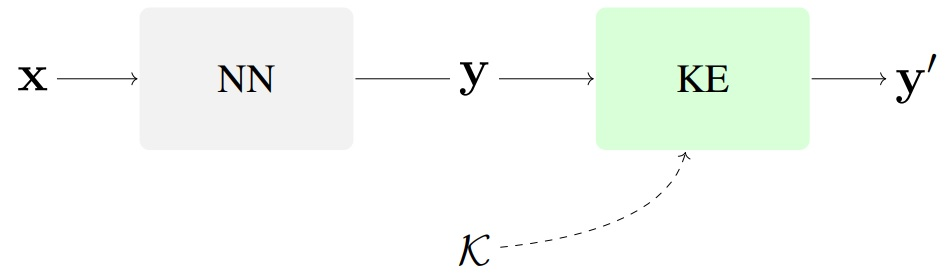
\includegraphics[width=.7\linewidth]{kenn_architecture.jpg}
    \caption{ Architecture of KENN - Features $ x $ are given in input to a neural network (NN), the predictions $ y $ are modified by the Knowledge Enhancer (KE) to satisfy a logical KB ($ \kappa $), thus obtaining the final predictions $ y'$. (Source:~\cite{kenn})}
    \label{fig:kenn_architecture}
\end{figure}

\paragraphn{Components}
As we can see from the Figure~\ref{fig:kenn_architecture}, the main component of the architecture is the Knowledge Enhancer, which has a specific role and is composed of a set of subcomponents that cooperate:
\begin{itemize}
    \item \textbf{Knowledge Enhancer (KE):} The KE is the layer responsible for injecting logical knowledge into the model. Given a logical KB $K$ composed of $n$ clauses, the KE contains $n$ independent \textit{Clause Enhancers} that produce $n$ variations to modify $y$ accordingly to $K$. These variations, also called deltas, are aggregated by the KE to obtain the enhanced output $y'$.
    \item \textbf{Clause Enhancer (CE):} The CE is the unit responsible for increasing the satisfaction of a clause by applying a \textit{boost function}, which acts on the predictions of the labels related to the literals of the clause. Each CE is associated to a clause weight $w_c$ that regulates the influence of the clause during the enhancement process.
    \item \textbf{T-conorm boost function (TBF):} The TBF is the function applied by each CE to increase the value of the Gödel t-conorm of its grounded clause. The TBF produces the deltas that will be aggregated by the KE to obtain the final predictions. Since the TBF is based on the Gödel t-conorm, which is non-differentiable, the authors propose the following soft differentiable approximation to compute the deltas:
    \begin{equation} \label{eq:tbf}
    	\delta _{w_{c}}(v)_{i} = w_{c} \cdot softmax(v)_{i}
    \end{equation}
    where $ w_{c} $ is the weight of the clause $ c $, $ v $ is the preactivation vector (i.e., the output of the base neural network) of the literals belonging to $c$, and $ i $ refers to the \textit{i-th} literal of the clause.
\end{itemize}

\paragraphn{Clause Enhancer details}
Now that the high-level architecture has been presented, we can go deeper into the details of the clause enhancement mechanism. Referring to Figure~\ref{fig:clause_enhancer}, the functioning of a CE can be summarized with the following steps:
\begin{enumerate}
    \item Receive the preactivations $ z $ of all the grounded literals (i.e., the output $y$ of the base neural network).
    \item Apply a pre-elaboration step $ \phi $ to filter the preactivations: keep only the preactivations of the literals belonging to the clause $ c $ and change the sign of the preactivations of negated literals.
    \item Apply the TBF (Equation \ref{eq:tbf}) to the resulting preactivations to produce the deltas.
    \item Apply a post-elaboration step $ \phi' $ to convert the TBF’s results into changes to be applied to the original preactivations $ z $: expand back the dimensionality by filling with 0s the positions of the previously filtered out preactivations, then change back the sign of the deltas of negated literals.
\end{enumerate}
An example of clause enhancement that may help to better comprehend the mechanism is shown in Figure~\ref{fig:example_enhancement}. 
\begin{figure}[H]
    \centering
    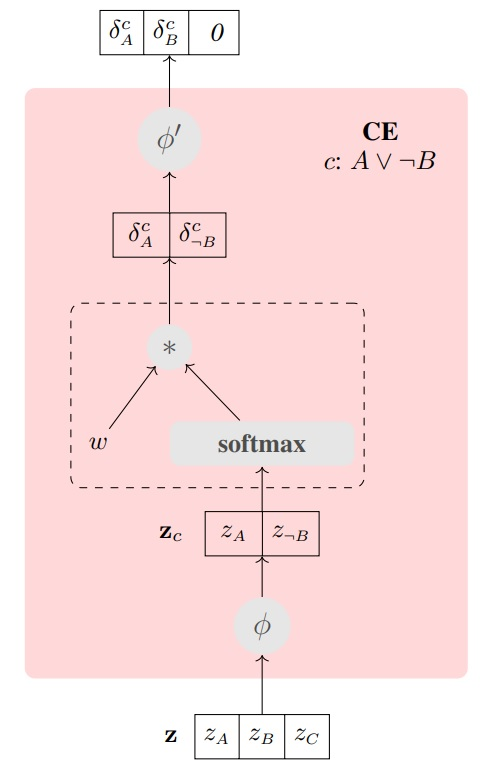
\includegraphics[width=.35\linewidth]{clause_enhancer.jpg}
    \caption{Clause Enhancer for $ A \vee \neg B $. (Source:~\cite{kenn})}
    \label{fig:clause_enhancer}
\end{figure}

\begin{figure}[H]
    \centering
    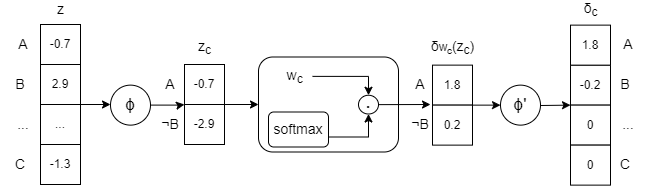
\includegraphics[width=.75\linewidth]{example_enhancement.png}
    \caption{Example of clause enhancement for $ A \vee \neg B $, with $w_{c}=2.0$}
    \label{fig:example_enhancement}
\end{figure}

\begin{figure}
    \centering
    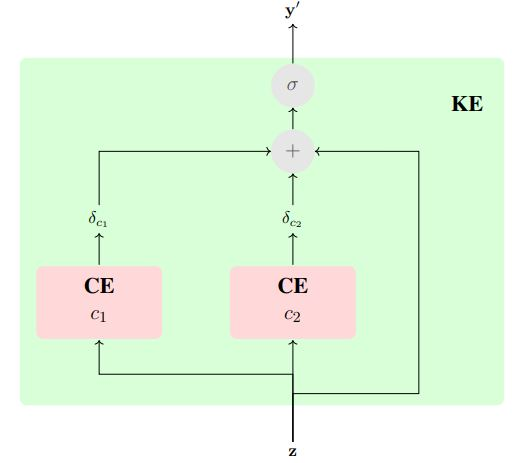
\includegraphics[width=.5\linewidth]{knowledge_enhancer.jpg}
    \caption{Knowledge Enhancer producing enhanced predictions. The deltas of each CE are summed to the preactivations of the base neural network. (Source:~\cite{kenn})}
    \label{fig:knowledge_enhancer}
\end{figure}

\paragraphn{Aggregation step}
Once understood the enhancement mechanism for a single clause, it is necessary to explain how the outputs of each CE are combined. An illustration of this step is available in Figure~\ref{fig:knowledge_enhancer}. As we can see, the KE aggregates the initial preactivations to the deltas coming from each CE. The aggregation consists of a simple sum and the resulting value is passed through an activation function to obtain the final predictions $y'$. The authors of KENN motivate the choice of the sum as it leads to faster learning and inference, thus resulting in higher scalability. However, this kind of aggregation may lead to the so-called \textit{conflicts}.

A conflict occurs when the same literal appears with different signs in two or more clauses, thus leading the CEs to produce for the same literal both positive and negative deltas. The natural consequence is that there could be side effects when performing the aggregation step since the benefits of a clause could be mitigated or completely overwhelmed by the effects of another clause. To better understand this particular situation, imagine having two clauses $ c_{1}: \neg A \vee B $ and $ c_{2}: \neg B \vee C \vee D $, where $B$ is the literal involved in possible conflicts. Let us assume that starting from an arbitrary preactivation vector $ z $ the CEs generate $ \delta (z_{c_{1}})_{B} = 0.7 $ and $ \delta (z_{c_{2}})_{B} = -0.5 $. At this point, we can aggregate the deltas obtaining $\delta _{B} = 0.7 - 0.5 = 0.2$. The result is that the final change on $ B $ will reflect the effect of the stronger grounded clause lowered by the effect of the weaker one. It is important to underline that the more literals involved in a clause, the less the probability to encounter relevant conflicts, since the same literal must be dominant in both clauses~\cite{kenn}.

\paragraphn{Enhancement of a logical implication}
An important aspect to remark and keep in mind is that since the goal of KENN is to increase the Gödel t-conorm of a grounded clause, the action of a CE is always the following: \textit{produce a positive boost to the preactivations of positive literals and a negative boost to the preactivations of negative literals}. In other words, the sign of a delta computed by the CE reflects the sign of the related literal of the clause. Thus, reminding that a logical implication must be expressed in KENN by using the logical equivalence $ A \to B = \neg A \vee B $, the effect of a CE always results in a decrease of the preactivation of $A$ and an increase of the preactivation of $B$. This means that a violated grounded clause (i.e., $ 1 \to 0 $) is always pushed by KENN towards its satisfiability (i.e., $ 1 \to 1 $, $ 0 \to 0 $, or $ 0 \to 1 $).

If we consider again the example in Figure~\ref{fig:example_enhancement}, which is based on the clause $A \vee \neg B $ that can be seen as $ B \to A $, we can analyze how the knowledge enhancement of an implication would modify the initial predictions. Table~\ref{tab:example_tbf_values} reports the values obtained at each step of the CE, plus the prediction on $A$ and $B$ before and after the enhancement. If we consider $ threshold = 0.5 $ to assign 1 and 0 to the grounded literals and we compare the columns $ \sigma (z) $ and $ \sigma (\delta _{w_{c}}(z)+ z)$, we can observe that KENN changed $1 \to 0$ into $1 \to 1$.

\begin{table}[h]
\centering
\caption{Numeric example of the action of KENN for $ A \vee \neg B $}
\label{tab:example_tbf_values}
\begin{tabular}{c|c|c|c|c|c|c|c|}
\cline{2-8}
                                 & $ z $ & $ \sigma (z) $       & $ z_{c} $ & $ \delta _{w_{c}}(z_{c}) $ & $ \delta _{w_{c}}(z) $ & $ \delta _{w_{c}}(z) + z $ & $ \sigma (\delta _{w_{c}}(z)+ z)$ \\ \hline
\multicolumn{1}{|c|}{$ A $}      & -0.7  & 0.33 ($ \approx 0 $) & -0.7      & 1.8                        & 1.8                    & 1.1                        & 0.75 ($ \approx 1 $)              \\ \hline
\multicolumn{1}{|c|}{$ B $}      & 2.9   & 0.95 ($ \approx 1 $) & -         & -                          & -0.2                   & 2.7                        & 0.94 ($ \approx 1 $)              \\ \hline
\multicolumn{1}{|c|}{$ \neg B $} & -     & -                    & -2.9      & 0.2                        & -                      & -                          & -                                 \\ \hline
\end{tabular}
\end{table}


\paragraphn{Considerations on the clause weight}
In the example above, KENN with its intervention changed the final predictions leading to a satisfied clause. This is not always the case, since the choice of a different clause weight could lead to another outcome. In Figure~\ref{fig:sigmoid_example} we can see two examples that start from the same preactivations, but use different clause weights. The examples show in a graphical way the changes introduced by KENN to the initial prediction from the perspective of the sigmoid activation function. Considering that a classification threshold of 0.5 on post-sigmoid values is equivalent to using a 0 threshold directly on preactivations, we can see that the delta produced in Figure~\ref{fig:sigmoid_example_w2} is not enough to push the prediction over the threshold. On the contrary, Figure~\ref{fig:sigmoid_example_w1} shows that the prediction changes its sign thanks to a higher clause weight.

\begin{figure}[h]
     \centering
     \begin{subfigure}{0.47\textwidth}
         \centering
         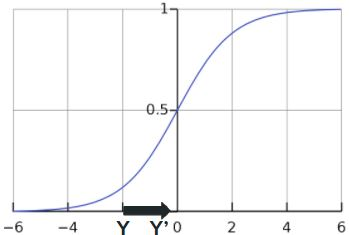
\includegraphics[width=\textwidth]{figures/ex_enhancement_w2.JPG}
          \caption{$w=2$,  $\delta_{Y} = 1.6$,  $Y'=-0.4$}
         \label{fig:sigmoid_example_w2}
     \end{subfigure}
     \hfill
     \begin{subfigure}{0.47\textwidth}
         \centering
         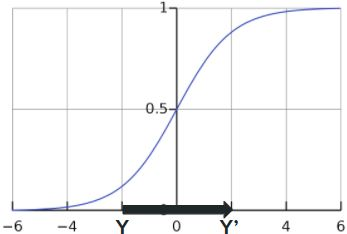
\includegraphics[width=\textwidth]{figures/ex_enhancement_w5.JPG}
         \caption{$w=5$,  $\delta_{Y} = 4$,  $Y'=2$}
         \label{fig:sigmoid_example_w1}
     \end{subfigure}
        \caption{Example of enhancement given $Y = -2$ and $softmax_{Y} = 0.8$, from the perspective of the sigmoid activation function}
        \label{fig:sigmoid_example}
\end{figure}

% \begin{table}
% \centering
% \caption{Truth table of the clause $ A \vee \neg B $}
% \label{tab:example_tbf_tt}
% \begin{tabular}{c|c|c|c|}
% \cline{2-4}
%                         & $ A $ & $ B $ & $ A \vee \neg B $ \\ \hline
% \multicolumn{1}{|c|}{1} & 0     & 0     & 1                 \\ \hline
% \multicolumn{1}{|c|}{2} & 0     & 1     & 0                 \\ \hline
% \multicolumn{1}{|c|}{3} & 1     & 0     & 1                 \\ \hline
% \multicolumn{1}{|c|}{4} & 1     & 1     & 1                 \\ \hline
% \end{tabular}
% \end{table}
\paragraphn{Relational KENN}
The authors of KENN propose also an extended version of the framework to use logical knowledge in relational domains. In that version, it is possible to specify relations between examples in contexts like collective classification by using binary predicates. The architecture of the relational version is slightly different and requires more sophisticated steps to inject logical knowledge into the neural network. The details can be found in~\cite{daniele2021neural} and will not be discussed here since this thesis focuses on the use of unary predicates.